\documentclass[conference]{IEEEtran}
\IEEEoverridecommandlockouts
% The preceding line is only needed to identify funding in the first footnote. If that is unneeded, please comment it out.
\usepackage{cite}
\usepackage{amsmath,amssymb,amsfonts}
\usepackage{algorithmic}
\usepackage{algorithm}
\usepackage{graphicx}
\usepackage{textcomp}
\usepackage{xcolor}
\usepackage{enumitem}
\usepackage{booktabs}
\usepackage{tabularx}
\usepackage{pifont}
\usepackage{titlesec}
\usepackage{balance}
\usepackage{tablefootnote}
\def\BibTeX{{\rm B\kern-.05em{\sc i\kern-.025em b}\kern-.08em
    T\kern-.1667em\lower.7ex\hbox{E}\kern-.125emX}}
\begin{document}

\title{ZhuLong: An Execution-Grounded Self-Evolving Agent for EDA Scripting}

\author{}

\maketitle

\begin{abstract}
Applying large language models to EDA scripting is difficult because the
relevant tool APIs are under-documented, sparsely represented in training
data, and judged only by real execution against hidden tests. We present
\textbf{ZhuLong}, an execution-grounded LLM coding agent for the pyAether
EDA platform that keeps the model frozen and solves tasks through a harness of
retrieval, documentation, and sandbox-execution tools, with a
precision-optimized static checker that catches deterministic API misuse
with no observed false positives. On top of this harness, an offline self-evolution
system distills execution traces into a governed three-tier memory store,
where every stage carries a reliability gate and a held-out evolution loop
rejects degrading rounds, and structural anti-leakage retrieval designed to prevent
cross-split answer copying. On the 158-task EDA-Eval-PyAether benchmark, the
full harness reaches 92.4\% pass@1 and transfers across LLM backbones. On a
harder, instance-disjoint challenge test, self-evolution from a bare start,
with all hand-written experience removed, surpasses the human-experience
baseline at 80.0\% vs.\ 77.5\% pass@1, and ablations isolate the contribution of each
governance gate and retrieval mechanism.
\end{abstract}

\begin{IEEEkeywords}
LLM Agents for EDA, EDA Scripting, Code Generation, Sandbox Execution, Self-Evolving Agents
\end{IEEEkeywords}

\section{Introduction}
\label{sec:introduction}

Large language models (LLMs) have demonstrated strong capabilities in
general-purpose code generation~\cite{wu2025openroad}, yet applying them to
electronic design automation (EDA) scripting remains difficult. EDA engineers
routinely write Python scripts that drive a commercial tool's API surface to
query designs, create layout instances, and manipulate netlists. These APIs
are tool-specific, sparsely documented, and generated through SWIG (Simplified Wrapper and Interface Generator) bindings
whose type rules differ from native Python. A general-purpose LLM can often
draft plausible code, but the code fails at runtime because it calls a
non-existent API, passes a native value where a SWIG-wrapped type is required,
or simply does not satisfy the task's hidden test.

Three obstacles make this setting harder than ordinary code generation.
First, the relevant APIs form a long tail that is under-represented in
training data, so the model must recall and inspect them at inference time
rather than from memory. Second, correctness cannot be judged statically: the
code must be executed against a real EDA environment to observe whether it
produces the intended side effect, and a syntactically valid call can still be
semantically wrong. Third, an agent that solves a task once does not thereby
learn to solve related tasks, unless its experience is externalized and
re-injected~\cite{wang2023voyager,zhao2024expel}, which risks injecting
misleading knowledge if that experience is not
governed~\cite{zhao2024expel,yang2026skillopt}.

We present \textbf{ZhuLong}, an execution-grounded LLM coding agent for
pyAether, the Python binding of the Aether EDA platform. ZhuLong keeps the
model frozen and solves tasks through a harness of MCP (Model Context Protocol) tools that retrieve
APIs, inspect documentation, and execute code in an isolated sandbox, with a
domain-level static checker that catches deterministic API misuse before
submission. On top of this harness, an offline self-evolution system distills
execution traces into reusable knowledge and re-injects it on later tasks,
under reliability gates that prevent ungoverned experience from misleading
the agent. The system is evaluated on EDA-Eval-PyAether, a benchmark of 158
real-world scripting tasks judged by real sandbox execution with hidden tests.

Our contributions are as follows.
\begin{itemize}[leftmargin=*]
\item A hardened harness substrate for frozen-agent EDA scripting, combining
dual-path API retrieval, documentation
enrichment, multi-port sandbox isolation, and a precision-optimized static
checker that catches deterministic misuse with no observed false positives
(Section~\ref{sec:method}).
\item A governed self-evolution system that distills execution traces into a
three-tier memory store with reliability gates at every stage, including
ground-truth anchoring, conditioned reflection with a scope-boundary design,
disconfirmation gating, a held-out evolution loop that rejects degrading
rounds, and structural anti-leakage retrieval that is designed to prevent cross-split
answer copying through names-only injection and deterministic docstring
generalization rather than relying on an evaluation gate
(Section~\ref{sec:selfev}).
\item An empirical study showing that the full harness reaches 92.4\% pass@1
on 158 tasks, and that self-evolution from a bare start surpasses the
hand-written experience baseline (80.0\% vs.\ 77.5\%) on a harder,
instance-disjoint challenge test, with ablations isolating the contribution
of each design choice (Section~\ref{sec:experiments}).
\end{itemize}

\section{Related Work}
\label{sec:related_work}

\subsection{LLM for EDA}
\label{sec:rw_eda}

LLMs for chip design have largely targeted RTL generation: ChipNeMo, RTLCoder, AutoChip, and CodeV-R1~\cite{liu2023chipnemo,liu2024rtlcoder,thakur2023autochip,zhu2026qimeng}
domain-adapt or fine-tune models for Verilog, relying on human-constructed
testbenches, which is orthogonal to operating an EDA tool's API surface.
The procedural-scripting strand ZhuLong belongs to has grown quickly:
ChatEDA, ChaTCL, EDA-Copilot, iScript, FluxEDA, and
AutoEDA~\cite{wu2024chateda,rui2025chatcl,xiao2025eda,xu2026iscript,chen2026fluxeda,lu2025autoeda}
span flow planning, Tcl/Q\&A assistance, single-turn generation, and execution
infrastructure. The closest is OpenROAD~Agent~\cite{wu2025openroad}, which
adds execution-feedback self-correction on an open physical-design tool, but
finetunes the model and does not externalize cross-task experience. Our scenario shares its
generate-execute-revise shape yet keeps the model frozen and judges pass/fail
by real sandbox execution with hidden tests. The Agentic EDA
survey~\cite{zang2025dawn} situates this line at L3 autonomy. Two gaps recur
for a frozen-agent, hidden-test setting: none externalizes cross-task
experience into a governed, leakage-controlled store, and none carries a
domain-level static check beyond the tool's own schema.

\subsection{Self-Evolving Agents with Governed Memory}
\label{sec:rw_self_evolving}

A broad family equips agents with reusable external memory: skill
libraries, cross-task insight distillation, hierarchical memory, and
cognitive architectures~\cite{wang2023voyager,zhao2024expel,packer2023memgpt,sumers2023cognitive},
with CodeAct~\cite{wang2024executable} unifying the action space as executable
Python. These assume an open world or a train/test-disjoint split, which
sidesteps the same-task regression signal our fixed-set setting must surface.
Treating the skill store as an optimization target, SkillOpt~\cite{yang2026skillopt}
edits a single skill document under a held-out gate and observes that
``plausible textual diagnoses can still hurt,'' echoing our concern that
ungoverned experience misleads. SkillOS~\cite{ouyang2026skillos} learns
curation via RL with a four-dimensional judge, and a same-named
Trace2Skill line distills trajectories: Ni~et~al.~\cite{ni2026trace2skill}
into a single skill directory, Du and Pinckney~\cite{du2026trace2skill} via
verifier-guided per-task evolution. These optimize one document on disjoint
splits with relatively dense signal, whereas our sparse-pass/fail, fixed-set
setting makes which-experience-to-trust more pressing than how to edit a
document.

Verifier-guided evolution brings the reward signal closer to our hidden-test
setting. ReVeal~\cite{jin2025reveal} self-generates test cases for dense
rewards, but self-generated tests can be gamed and do not substitute for a hidden verifier.
The Du variant of Trace2Skill shares our hidden-verifier, no-answer framing
but runs online per task with physical isolation and task-wise skills. Its
finding that cross-task transfer is unreliable for heterogeneous RTL cautions
how far logical-error knowledge should travel. EvoAgentBench~\cite{gao2026evoagentbench},
the most comparable benchmark, formalizes this tension with an
ability-supported yet instance-disjoint split, finding that an Anchor Skill
oracle helps while no automatic method sustains the gain.

Finally, VeriHarness~\cite{ray2026structured} shows that structured feedback
improves repair, and several works
inform the governance machinery: MUSE-Autoskill~\cite{lin2026muse} and
MemOrb~\cite{huang2025memorb} on refinement and reflection,
AHE~\cite{lin2026agentic} on tools and middleware carrying improvement,
Externalization~\cite{zhou2026externalization} and
Reflexion~\cite{shinn2023reflexion} on memory artifacts and same-task
iteration, Governing Evolving Memory~\cite{lam2026governing} on System-2
verification, and SWE-bench~\cite{jimenez2024swe} on code-agent evaluation.
The recurring lesson is that an evolving memory needs an external,
ground-truth-anchored gate to stay trustworthy, which under sparse pass/fail
and an anti-leakage constraint is the question our method takes up.

\section{Method}
\label{sec:method}

\begin{figure*}[t]
\centering
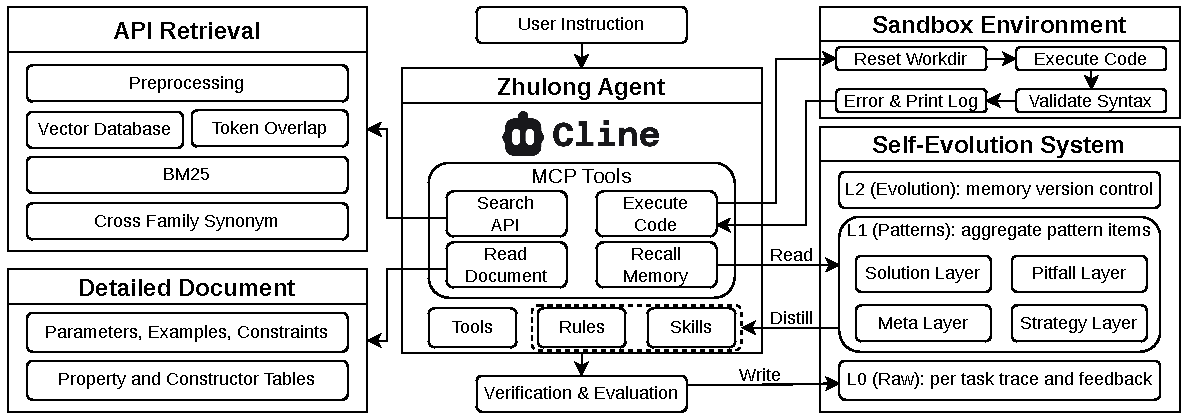
\includegraphics[width=1.0\textwidth]{figures/zhulong.pdf}
\caption{ZhuLong system architecture.}
\label{fig:architecture}
\end{figure*}

ZhuLong targets pyAether, the Python binding of the Aether EDA platform, whose APIs are exposed through SWIG bindings and span a long tail of tool-specific, often under-documented call sites. The overall architecture is shown in Figure~\ref{fig:architecture}. Before studying the self-evolution layer, we harden the harness substrate itself, which comprises three components: API retrieval (Section~\ref{sec:method_retrieval}), documentation enrichment (Section~\ref{sec:method_doc}), and sandbox execution (Section~\ref{sec:method_sandbox}).

\subsection{API Retrieval}
\label{sec:method_retrieval}

Our MCP server exposes two recall tools: a semantic path (\texttt{search\_apis}) and a keyword path (\texttt{search\_apis\_by\_keyword}). The first path embeds only the API name and a short summary, because embedding the full page would push the target API toward documentation noise. To cover matches the summary misses, a BM25 pass over the full description text is appended as a supplement. The agent reads provenance from a \texttt{source} field.

The second path is the complementary path for queries the semantic index handles poorly, such as abbreviations (CV), camel case fragments (dbCrtInst), or when the agent wants a different angle. To make such fragments addressable, the index and the query are tokenized the same way: each API name is split on camel case boundaries with the family prefix (\texttt{ae}/\texttt{db}/\texttt{pyAether.}) stripped first, so \texttt{dbOpenCV} yields \texttt{Open} and \texttt{CV} rather than a \texttt{dbOpen} fragment, and matching is case-insensitive. The query is then bidirectionally expanded for abbreviations (abbr.$\to$full, e.g.\ CV$\to$CellView, and full$\to$abbr., e.g.\ create$\to$crt), so the keyword can match the abbreviated tokens inside API names.

A query is first routed by classifying into abbreviation, fragment, or natural-language. The last triggers a soft redirect that appends semantic results so an agent that misused the keyword tool for a natural-language query still sees both angles, and a fragment that is itself a full API name short-circuits to an exact-match hint directing the agent to read the full API document rather than re-searching.

Finally, a cross-family synonym map links the four API families that expose functionally equivalent operations (the procedural db* database layer, the object-oriented emy* wrapper, the goa* geometry layer, and the ae* Aether layer) and appends the equivalents of any hit. For example, hitting \texttt{dbCrtRect} also surfaces \texttt{emyRect.create}, addressing the failure mode where an agent recalls the correct family but picks the wrong interface style.

% \begin{algorithm}[t]
% \caption{Keyword recall with heterogeneous-score tiering}
% \label{alg:keyword}
% \begin{algorithmic}[1]
% \REQUIRE query $q$, top-$k$, API index $\mathcal{I}$ (name tokens + BM25 corpus)
% \STATE $t \leftarrow \textsc{ClassifyQuery}(q)$ \COMMENT{abbr. $|$ fragment $|$ NL}
% \STATE $Q \leftarrow \textsc{TokenizeBidir}(q)$ \COMMENT{camelCase split + abbrev.\ expand, both directions}
% \STATE $\mathcal{N} \leftarrow \textsc{NameOverlap}(\mathcal{I}, Q)$ \COMMENT{$F_2\in[0,1]$, $\beta{=}2$}
% \STATE $\mathcal{B} \leftarrow \textsc{BM25}(\mathcal{I}, Q)$ \COMMENT{score $\in[0,30^+]$, filter $<1.0$}
% \STATE $\mathcal{L}_1 \leftarrow \{r \in \mathcal{N} : r.s \geq 0.5\}$ \COMMENT{exact, tier 1}
% \STATE $\mathcal{L}_2 \leftarrow \{r \in \mathcal{N} : 0.2 \leq r.s < 0.5\}$ \COMMENT{weak, tier 2}
% \STATE $\mathcal{L}_3 \leftarrow \mathcal{B} \setminus \mathcal{N}$ \COMMENT{BM25-only, tier 3}
% \STATE boost each $r \in \mathcal{L}_2$ that also appears in $\mathcal{B}$ \COMMENT{dual-hit, no re-score}
% \STATE $\mathcal{R} \leftarrow \mathcal{L}_1 \;\Vert\; \mathrm{sort}(\mathcal{L}_2) \;\Vert\; \mathrm{sort}(\mathcal{L}_3)$ \COMMENT{tier concat., not score merge}
% \STATE append cross-family synonyms of $\mathcal{R}_{1..k}$, tagged, outside top-$k$
% \IF{$t =$ NL}
%   \STATE append semantic results, tagged \texttt{vector\_redirect}
% \ELSIF{$t =$ fragment $\land\; q \in \mathcal{I}$}
%   \STATE prepend $\{q, s{=}1.0, \texttt{exact\_match}\}$
% \ENDIF
% \STATE tag every $r$ with its \texttt{source} and return $\mathcal{R}$
% \end{algorithmic}
% \end{algorithm}

\subsection{Documentation Enrichment}
\label{sec:method_doc}

The reference API database ships per-API signature pages but omits one thing EDA scripting needs: instance properties of its classes. We close this gap by parsing the raw documentation into a property table and append it to each detailed response, so a queried class exposes its instance attributes alongside its methods. Constructor notes also disambiguate ambiguous calls: for example, \texttt{emyPointArray} accepts a plain list of points, a fact the per-signature page does not state.

\subsection{Sandbox Execution}
\label{sec:method_sandbox}

We run multiple isolated sandbox endpoints, each with an independent working directory, and dispatch requests through a queue pool. A routine clears working directories before each run and resets library files to minimal content, so a prior run's leftover library state does not bias the next.
Because pyAether's SWIG bindings expose all symbols at import time regardless of whether the underlying function exists at runtime, the import succeeds and ordinary Python syntax and name checks see every call as valid regardless of whether the underlying API exists or accepts the given arguments. As a result, a call the agent never validates in its self-test raises no error at sandbox time, yet fails the hidden test that exercises that path. After execution, our checker extracts every API call with its arguments and checks each against the API document:
\begin{itemize}
\item \textbf{Fabricated API}: the code calls a non-existent API
\item \textbf{Wrong keyword argument}: a keyword argument name does not match any documented API parameter
\item \textbf{Native value for a SWIG type}: a keyword argument receives a native Python value (e.g., a plain \texttt{str} or \texttt{tuple}) where the API documents a SWIG-wrapped type
\item \textbf{Failure ignorance}: except block which swallows an error
\end{itemize}
The checker runs after code execution: when the agent's run reports no
error, the code is checked and error-level findings are appended to the
response the agent reads. The rules are derived from the API documentation
and refined through extensive testing against real submissions, and the
checker is held to a hard constraint of no observed false positives, so it never flags a
task that would otherwise pass.


\section{Self-Evolution}
\label{sec:selfev}

The substrate of Section~\ref{sec:method} solves individual tasks, but it does not let the agent improve across tasks. ZhuLong adds an offline self-evolution system (the right side of Figure~\ref{fig:architecture}) that distills execution traces and evaluation results into reusable knowledge and re-injects it into later tasks. Knowledge is organized in three tiers, following the episodic-semantic-procedural memory distinction of cognitive architectures for language agents~\cite{sumers2023cognitive}: \emph{L0} holds raw per-task trace artifacts (episodic), \emph{L1} is the aggregated pattern store (semantic), and \emph{L2} archives distilled skill versions (procedural). Within L1, patterns are partitioned into four layers by the kind of knowledge they carry: a \emph{solution} layer of verified API routes from passed tasks, a \emph{pitfall} layer of negative warnings from failed tasks, a \emph{meta} layer of effective query patterns, and a \emph{strategy} layer of decision records. The layer tag travels with each entry and lets retrieval filter by knowledge type, so that, for example, pre-injection can admit the solution layer while routing pitfalls to the runtime query (Section~\ref{sec:se_read}). Two design points govern when each side acts. The \emph{write} side runs once per round, offline, after a training batch has been evaluated. The \emph{read} side fires at two points: a per-task pre-injection at task formatting, which recalls relevant L1 patterns into the prompt, and an on-demand runtime query, which the agent invokes when it hits an error.

The guiding principle is governance, not accumulation: experience that looks plausible can still mislead, since a verified entry carrying the agent's own incorrect inference is worse than no entry. This is an instance of the finding that plausible but ungoverned experience can hurt~\cite{zhao2024expel,yang2026skillopt}. Every stage below therefore carries a reliability gate. The write side (Sections~\ref{sec:se_distill}--\ref{sec:se_govern}) proceeds in pipeline order, the read side is Section~\ref{sec:se_read}, and the outer loop is Section~\ref{sec:se_loop}. An offline LLM performs all reflection and judgment.

\subsection{Distillation and Reflection}
\label{sec:se_distill}

The write side turns a trace into a trustworthy \emph{L0} artifact and routes each failed task to the reflection path whose input semantics match. The reflection engine then produces \emph{L1} pattern entries under constraints that prevent mislead-prone inferences from being generated in the first place.

A trace's own success signal is unreliable, because the agent's self-report overestimates the true pass rate. We therefore override it with the evaluator's binary verdict before any reflection begins. This establishes the reliable feedback signal that Reflexion identifies as necessary for reflection to help rather than harm~\cite{shinn2023reflexion}. A verified entry is anchored to the APIs the submitted code called, not those it merely fetched.

A task that still errors on its final attempt has a genuine, unfixed failure and takes the error path, anchored on its last error. A task whose final self-test passed but that the evaluator failed with an empty error log, takes the contradiction path instead. The split matters because for a self-test-passed task the error log holds only stale, already-repaired errors, and mining pitfalls from these would record bugs the agent already solved. On the contradiction path the reflection LLM receives only the task specification, the submitted code, and evaluation output, and is asked to find a single contradiction between specification and observed behavior. An offline branch-coverage analysis supplies deterministic evidence: functions never executed and API calls never reached.

Each \emph{L1} entry carries a reliability tier applied by the system: \emph{verified} (passed task), \emph{unverified} (failed task, direction LLM-judged correct), or \emph{pitfall} (negative warning). A verified entry states not just what worked but under which observable conditions: a precondition and a constraint drawn only from trace facts. Negative warnings obey a phrasing rule: never an absolute ``avoid~X,'' always a conditional ``X~requires~Y, recovered by the action the code actually took.'' An absolute prohibition is too easily read as a blanket interdiction.

\subsection{Governed Knowledge Lifecycle}
\label{sec:se_govern}

Extracted \emph{L1} patterns enter a lifecycle of aggregation, reliability gating, aging, and gated promotion to the always-on rule and on-demand skill layers.

ExpeL shows that failures carry more information than successes when judging learned insights~\cite{zhao2024expel}, but leaves this to unweighted vote counting. We make the attribution precise: A \emph{verified} entry is disconfirmed by a failed task only when the failure is an API misuse and the failing API is precisely attributed to the entry's primary API by parsing the error. At a count of two or more the entry is flagged on injection and, strictly, filtered out before promotion to rules or skills. Aggregation respects a trust-anchor guard, an \emph{unverified} trace can never downgrade a \emph{verified} entry, and aging is demote-not-delete: a verified entry not re-confirmed for five rounds drops to unverified, reversibly.

Two quality mechanisms guard promotion to rules and skills, both adopted from prior work: a four-dimensional judge (abstraction, reusability, actionability,
faithfulness) following SkillOS~\cite{ouyang2026skillos}, and a MUSE-style create-evaluate-refine loop~\cite{lin2026muse} that rewrites low-scoring skills before any deprecation. Our contribution is the gates around these: a zero-exception generality gate rejects any candidate rule whose always/never statement does not hold across the entire API surface.

\subsection{Anti-Leakage Retrieval}
\label{sec:se_read}

The read side governs how a downstream agent consumes distilled knowledge. Under an instance-disjoint split, a held-out task that recalls a training sibling's verbatim API sequence would copy its answer rather than transfer its method. Trace2Skill prevents this by sanitizing the feedback the agent sees~\cite{du2026trace2skill}. We adopt the goal but realize it structurally on the retrieval side, through four mechanisms: three for the solution layer and a routing rule that keeps pitfalls out of pre-injection.

\textbf{Names-only pre-injection.}
A solution entry is reduced to the set of API names it mentions, dropping call order, parameters, and sequence, so a held-out task learns only ``these APIs are relevant,'' not how to call them. The rationale is that a full call sequence over-specifies: it tempts the agent to copy a sibling's solution rather than adapt the route to its own task.

\textbf{Deterministic docstring generalization.}
A shared regular-expression stripper removes task-identifying specifics (quoted literals, instance names, coordinates, mode flags) from the docstring on both the distillation and query sides, so same-family tasks produce identical generalized text and transfer at the family level without verbatim leakage. Determinism is the point: the same function must run on both sides so
that a task's query matches the embedding its sibling produced, and an LLM canonicalizer could silently mismatch the two sides and break the match undetected.

\textbf{Embed the problem, return the solution.}
A solution entry is embedded under a generalized summary of the problem while the full API sequence is carried in metadata and returned only at read time, so retrieval matches on problem similarity and a sibling's solution is not buried by another sibling's similar solution text. This separates what the index matches on (the problem) from what the agent receives (the solution), so a harder task can still surface a relevant easier sibling's route without the easier sibling's exact sequence leaking.

\textbf{Pitfalls are not pre-injected.}
Pre-injecting pitfalls alongside solutions is unsound by construction: a task's description does not predict which API it will misuse, so a recalled pitfall is usually off-target. Pitfalls instead enter through the on-demand runtime query, where the agent's actual error is the retrieval key. This error-to-pitfall match is sound where a description-to-pitfall match is not.

\subsection{Held-Out Gated Evolution}
\label{sec:se_loop}

The outer loop chains write to read across rounds. After each training round, the agent generates on validation tasks, which never carry distillation, so the system never learns from validation, and the round's full evolved state is accepted only if the validation pass rate does not regress by more than a 5\% margin relative to the previous accepted round. Otherwise it is rolled back atomically from a snapshot. This extends the held-out acceptance criterion of SkillOpt~\cite{yang2026skillopt} from a single skill document to the entire evolved state, so validation tests the generalization of distilled knowledge rather than its memorization.


\section{Experiments}
\label{sec:experiments}

We evaluate ZhuLong on EDA-Eval-PyAether, a benchmark of 158 real-world pyAether scripting tasks. Each task is a natural-language docstring plus a function signature, and a submission passes only if real sandbox execution satisfies a hidden test (the black-box verifier). The primary model is
DeepSeek-V4-Pro-Preview.

The experiments fall into two parts. The first evaluates the full ZhuLong harness, which carries hand-written domain experience, on all 158 tasks, and asks three questions: does the full retrieval stack improve over a semantic-only baseline, does the hand-written experience (skills and rules
integral to the harness) earn its place, and does the harness transfer across LLM backbones. The second part then asks whether self-evolution, with the human experience removed, can surpass the same effect.

\subsection{Harness Evaluation}
\label{sec:exp_retrieval}

The retrieval layer has two levels: \emph{full} (the configuration of Section~\ref{sec:method_retrieval}) and \emph{semantic-only}, which keeps the semantic \texttt{search\_apis} path but disables the keyword tool and BM25 supplement. The experience layer has two levels: \emph{bare} (no skill, rule) and \emph{human}, the full ZhuLong configuration carrying four hand-written skills and one rule. The skills cover API search strategy, command family selection, a context degradation guard, and SWIG type construction. The rule enforces code-generation discipline. These hand-written assets were authored from broad domain expertise accumulated over the pyAether platform's development, not by inspecting or fitting them to the 158 benchmark tasks, so they do not constitute test-set leakage.
Table~\ref{tab:retrieval_ablation} reports the 2$\times$2 factorial over the retrieval and experience factors. Both factors are positively associated with pass@1: the full retrieval stack raises the pass rate under either experience level, and the hand-written experience raises it under either retrieval level.

\begin{table}[h]
\caption{Retrieval--experience decomposition on the 158-task benchmark (single run, DeepSeek-V4-Pro-Preview). Time is wall-clock per run, and tokens are summed over all tasks.}
\label{tab:retrieval_ablation}
\centering
% \small
\begin{tabular}{cccrr}
\toprule
Experience & Retrieval & Pass@1 & Time & Token \\
\midrule
bare  & semantic-only & 87.3\% & 15.0\,h & 83.1\,M \\
bare  & full          & 88.6\% & 15.8\,h & 75.3\,M \\
human & semantic-only & 89.9\% & 17.0\,h & 122.9\,M \\
human & full          & 92.4\% & 22.5\,h & 114.8\,M \\
\bottomrule
\end{tabular}
\end{table}

We choose Task~132 as an example to show the exact effect of the keyword-based search. Task~132 connects two orthogonal routing paths by placing a via at their intersection, which requires constructing several SWIG-wrapped types. Under
semantic-only retrieval the agent issued only natural-language queries such as ``get net from shape or path object'' and never surfaced the type names it needed, failing with a native tuple passed where construction was required.
Under full retrieval the agent queried the type names verbatim
(\texttt{ViaDef}, \texttt{emyPoint}, \texttt{emyString}) through the keyword path, whose camel case split and abbreviation expansion made them directly addressable. It then fetched their construction signatures and passed. The
contrast is exactly the keyword path's purpose: abbreviation-dense, camel case API names that a natural language query cannot embed against.

To validate the generalization of the ZhuLong harness, we run the same full-retrieval, human-experience configuration on four alternative LLMs (single run each, 158 tasks, Table~\ref{tab:cross_model}). pass@1 is positively associated with backbone capability: the stronger models stay close to the primary, consistent with a frozen harness transferring across model families. The weakest backbone (Doubao-Seed-2.0-pro, 71.5\%) also stands out on token usage, roughly a quarter of the others, which indicates it stops iterating early and under-uses the retrieve and execute loop rather than failing on the APIs it recalls. We therefore read its low pass rate as a base-capability limitation. The harness is model-agnostic, but the frozen agent still needs sufficient base capability to act on the retrieved APIs and sandbox feedback. Aggregating the 111~failures across the five backbones by the exception their sandbox execution raised (Figure~\ref{fig:failure_types}), the distribution is dominated by \texttt{AssertionError} (54.1\%): the code runs to completion with no thrown exception, but the hidden test asserts a property it does not satisfy. This is the class of failures no static check can reach, a logic or result error rather than a syntactic or type error, and it is consistent with the static checker intercepting deterministic API-misuse failures, but the majority of residual failures are semantic and require real execution to expose.

\begin{table}[h]
\caption{Cross model generalization: the same full-retrieval, human-experience configuration across five LLMs (single run, 158 tasks). Tokens are summed over all tasks.}
\label{tab:cross_model}
\centering
\small
\begin{tabular}{lcrr}
\toprule
Model & Pass@1 & Time & Token \\
\midrule
DeepSeek-V4-Pro-Preview   & 92.4\% & 22.5\,h & 114.8\,M \\
GLM-5.2           & 91.1\%          & 28.0\,h & 128.0\,M \\
Kimi-K2.6         & 89.2\%          & 22.7\,h & 126.2\,M \\
DeepSeek-V4-Flash-Preview & 85.4\%          & 11.1\,h & 134.0\,M \\
Doubao-Seed-2.0-pro   & 71.5\%          & 7.5\,h  & 28.3\,M \\
\bottomrule
\end{tabular}
\end{table}

\begin{figure}[h]
\centering
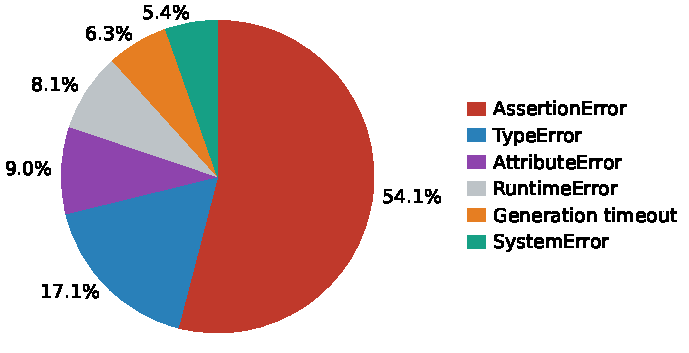
\includegraphics[width=\columnwidth]{figures/failure_type_distribution.pdf}
\caption{Distribution of failure types across the five LLM backbones on the
158-task benchmark (111~failures aggregated).}
\label{fig:failure_types}
\end{figure}

\subsection{Self-Evolution}
\label{sec:exp_selfev}

In this subsection, we ask whether self-evolution, with the human experience removed, can surpass the same effect. Since the bare agent already passes roughly 87\% of the 158 tasks, the ceiling dilutes the gap between methods into the sampling noise. Moreover, self-evolution distills knowledge from training tasks and risks overfitting them, and our held-out gating strategy needs a separate validation set. We therefore adopt an instance-disjoint \emph{challenge split} (train~98 / val~20 / test~40), in the spirit of EvoAgentBench's ability-supported yet instance-disjoint split~\cite{gao2026evoagentbench}, stratified so that the test set concentrates the more discriminative tasks, identified by their testbench code length and the number of unique APIs it uses. Because the validation and test sets are small, every self-evolution evaluation is the mean of \textbf{five} independent runs with its standard deviation.

Table~\ref{tab:sevolution} reports test pass@1 across rounds, against the bare baseline (no evolved knowledge) and the human baseline. Self-evolution clears the bare baseline by +14.0~pp
(66.0\%$\to$80.0\%) and surpasses the human baseline (80.0\% vs.\ 77.5\%) at round~2, after which round~3 regresses to 75.5\%. The validation trend is consistent: val peaks at round~2 (88.0\%) and drops at round~3 (80.0\%), so the gate accepts rounds~1 and~2 but rejects round~3, rolling back its 52 new entries and freezing the knowledge base at round~2 (334~entries, 20~skills). Crucially, the test trend now agrees with validation: round~3 also regresses on test (75.5\% vs.\ 80.0\%), confirming the gate's rejection was not a validation-specific artifact but reflected genuine overfitting. The stability improvement across rounds is also visible: round~2's $\pm$3.1 is the tightest spread, below the human baseline's $\pm$5.3.

\begin{table}[h]
\caption{Self-evolution on the challenge test set (40 tasks, 5 runs each, DeepSeek-V4-Pro-Preview). ``Patterns'' is the L1 entry count, ``skills'' are auto-distilled, and the held-out gate accepts R1/R2 and rejects R3.\tablefootnote{We do not show rules here because self-evolution does not distill any rule that passes the gate quality check.}}
\label{tab:sevolution}
\setlength{\tabcolsep}{4pt}
\centering
\footnotesize
\begin{tabular}{lcccc}
\toprule
Knowledge & Patterns & Skills & Pass@1 (test) & Pass@1 (val) \\
\midrule
bare          & 0   & 0  & 66.0\%$\pm$7.2  & --- \\
self-evolved R1 & 256 & 16 & 78.0\%$\pm$9.9  & 81.0\%$\pm$8.2 (accept) \\
self-evolved R2 & 334 & 20 & \textbf{80.0\%}$\pm$3.1  & 88.0\%$\pm$2.7 (accept) \\
self-evolved R3 & 386 & 25 & 75.5\%$\pm$6.7  & 80.0\%$\pm$3.5 (reject) \\
\midrule
human baseline & --- & 4  & 77.5\%$\pm$5.3  & --- \\
\bottomrule
\end{tabular}
\end{table}

With five runs, validation and test trends are consistent: round~2 peaks on both (88.0\% val, 80.0\% test) and round~3 regresses on both (80.0\% val, 75.5\% test), confirming the gate's rejection of round~3 reflects genuine overfitting rather than a validation-specific artifact.

To examine each gate's contribution to knowledge quality, we ablate each write-side gate introduced in Section~\ref{sec:se_distill}--\ref{sec:se_govern} (ground-truth anchoring, failure routing, the contradiction path, the scope boundary, and disconfirmation) by toggling it on and off and measuring the quality of the knowledge the write side produces. A full evolution round costs roughly 13~hours, and the failure-triggered gates fire on only a few tasks per round, so an end-to-end ablation per gate is both expensive and signal-starved. We instead freeze the 24~distinct failed-task traces accumulated across the post-split batches and re-run only the offline reflection chain with each gate toggled, measuring knowledge quality rather than end-to-end pass@1, in the spirit of the shared-trace-pool design of Trace2Skill~\cite{ni2026trace2skill}, which collects traces once and re-uses them across the cheap patch-proposal and merge stages. The test failure traces are used only as inputs to this offline reflection, and no knowledge produced from them is injected into any test evaluation, so their inclusion does not constitute test-set leakage. Table~\ref{tab:se_write_ablation} reports entry counts. Because the offline reflection LLM is not perfectly deterministic, the ON column (the full system) varies by one across gates. We read only the gate-shaped deltas, not
single-entry differences.

\begin{table}[h]
\caption{Write-side gate ablation on the frozen 24-task failure trace pool. ``ON'' and ``OFF'' are the number of L1 pattern entries the offline reflection produces with the gate enabled and disabled, respectively. The ON column varies by one across gates due to LLM non-determinism.}
\label{tab:se_write_ablation}
\centering
\footnotesize
\begin{tabular}{lccl}
\toprule
Gate & ON & OFF & Finding \\
\midrule
GT anchoring       & 37 & 48 & 12 false-positive verified (net +11) \\
contradiction path & 37 & 54 & 17 more but lower-precision entries \\
routing            & 36 & 37 & forced success path, no pitfalls \\
scope boundary     & 36 & 36 & not triggered on this pool \\
disconfirm filter  & 37 & 37 & not triggered on this pool \\
\bottomrule
\end{tabular}
\end{table}

The ablation isolates which gates earn their place. Ground-truth anchoring is
the strongest: without it, 12 of 24~tasks yield at least one falsely verified
entry, because the trace's self-report of success is trusted. The net entry
count rises by 11 (from 37 to 48) rather than by 12, because one of the 12
false-verified tasks would have produced no entry under correct anchoring
(its pitfall was never generated), so only 11 entries are net-added. The contradiction path for semantic failures trades quantity for
precision: disabling it forces those tasks onto the error path, which produces
17~more entries but of lower precision, since the error path mines pitfalls
from stale, already-repaired errors. Routing itself matters mainly through the
contradiction path it enables. Disabling routing forces all failed tasks onto the
success branch (as if they had passed), so no pitfalls are produced at all,
losing that knowledge entirely. The scope-boundary and disconfirmation
gates do not trigger on this 24-task pool, so their contribution cannot be
isolated here and is left unverified by this ablation.

\begin{table}[h]
\caption{Read-side injection ablation, frozen round-2 knowledge, validation (20 tasks, 5 runs). Each row varies one mechanism away from the full system (baseline 88.0\%$\pm$2.7).}
\label{tab:se_read_ablation}
\centering
\small
\begin{tabular}{lcc}
\toprule
Configuration & Pass@1 (val) & vs.\ Baseline \\
\midrule
baseline (full system)         & 88.0\%$\pm$2.7 & --- \\
pitfall pre-injection on       & 80.0\%$\pm$5.0 & $-$8.0~pp \\
docstring generalization off   & 81.7\%$\pm$5.8 & $-$6.3~pp \\
full-sequence injection        & 83.3\%$\pm$5.8 & $-$4.7~pp \\
embed solution (not problem)   & 88.0\%$\pm$2.7 & 0~pp \\
\bottomrule
\end{tabular}
\end{table}

We also ablate each of the four read-side mechanisms introduced in Section~\ref{sec:se_read} (names-only pre-injection, docstring generalization, the problem-side embedding, and the decision not to pre-inject pitfalls) by freezing the round-2 knowledge and
varying the injection configuration, then re-running the agent on validation (baseline 88.0\%$\pm$2.7). Table~\ref{tab:se_read_ablation} isolates each. The results support three of the four design choices and qualify the
fourth. Pre-injecting pitfalls is the most harmful ($-$8.0~pp): a task's description does not predict which API it will misuse, so a recalled pitfall is usually off-target, confirming the choice to route pitfalls through the runtime query instead. Docstring generalization ($-$6.6~pp when disabled) and names-only injection ($-$4.7~pp when the full sequence is injected) each contribute, the former because disabling it breaks the query--embedding symmetry, the latter because a full call sequence over-specifies and misleads. The embedding strategy (embedding the problem summary vs.\ the solution text) shows no measurable effect here. We attribute this to names-only injection, under which the retrieved content is the same regardless of what the entry was embedded on, so the embedding choice is dominated by the names-only
reduction. The problem-side embedding is therefore justified by its anti-leakage role rather than by a measurable pass@1 gain in this configuration.

\section{Conclusion and Future Work}

We presented ZhuLong, an execution-grounded LLM coding agent for pyAether
EDA scripting. The agent operates through a frozen harness of MCP tools for
API retrieval, documentation inspection, and isolated sandbox execution, with
a precision-optimized static checker that intercepts deterministic API misuse
with no observed false positives. On this substrate, an offline self-evolution system
distills execution traces into a three-tier memory store, governed by
reliability gates at every stage and a held-out evolution loop that rejects
degrading rounds. Structural anti-leakage retrieval is designed to prevent cross-split
answer copying on the retrieval side rather than relying on an evaluation
gate.

On the 158-task EDA-Eval-PyAether benchmark, the full harness reaches 92.4\%
pass@1, and the harness transfers across LLM backbones down to a
base-capability floor. On a harder, instance-disjoint challenge test,
self-evolution from a bare start, with all hand-written experience removed,
surpasses the human-experience baseline at 80.0\% vs.\ 77.5\% pass@1, with
validation and test trends agreeing that round~3 overfits. Ablations isolate the contribution
of each design choice: ground-truth anchoring prevents half of the failed
tasks from producing false-positive verified knowledge, and the read-side
mechanisms earn their place, with three of the four showing measurable gains and the fourth justified by its anti-leakage role, and pitfall pre-injection identified as the
most harmful when wrongly applied.

Several limitations remain. The challenge test set is small (40 tasks), so
per-run variance is nontrivial, but five runs per configuration establish
consistent validation and test trends. Two write-side gates
(scope boundary and disconfirmation) do not trigger on the available failure
pool, so their end-to-end contribution is left unverified by the ablation.
The self-evolution system is evaluated on a single EDA domain, and whether
the governance mechanisms transfer to more heterogeneous task distributions
is an open question. Future work will extend the evaluation to additional
EDA tool flows and larger task sets, and will investigate whether the
governed-memory principle applies to domains beyond EDA scripting.

\clearpage
\balance
\bibliographystyle{IEEEtran}
\bibliography{reference}

\end{document}
